%
% This is a borrowed LaTeX template file for lecture notes for CS267,
% Applications of Parallel Computing, UCBerkeley EECS Department.
% Now being used for CMU's 10725 Fall 2012 Optimization course
% taught by Geoff Gordon and Ryan Tibshirani.  When preparing 
% LaTeX notes for this class, please use this template.
%
% To familiarize yourself with this template, the body contains
% some examples of its use.  Look them over.  Then you can
% run LaTeX on this file.  After you have LaTeXed this file then
% you can look over the result either by printing it out with
% dvips or using xdvi. "pdflatex template.tex" should also work.
%

\documentclass[twoside]{article}
\setlength{\oddsidemargin}{0.25 in}
\setlength{\evensidemargin}{-0.25 in}
\setlength{\topmargin}{-0.6 in}
\setlength{\textwidth}{6.5 in}
\setlength{\textheight}{8.5 in}
\setlength{\headsep}{0.75 in}
\setlength{\parindent}{0 in}
\setlength{\parskip}{0.1 in}

%
% ADD PACKAGES here:
%

\usepackage{amsmath,amsfonts,graphicx}

%
% The following commands set up the lecnum (lecture number)
% counter and make various numbering schemes work relative
% to the lecture number.
%
\newcounter{lecnum}
\renewcommand{\thepage}{\thelecnum-\arabic{page}}
\renewcommand{\thesection}{\thelecnum.\arabic{section}}
\renewcommand{\theequation}{\thelecnum.\arabic{equation}}
\renewcommand{\thefigure}{\thelecnum.\arabic{figure}}
\renewcommand{\thetable}{\thelecnum.\arabic{table}}

%
% The following macro is used to generate the header.
%
\newcommand{\lecture}[4]{
   \pagestyle{myheadings}
   \thispagestyle{plain}
   \newpage
   \setcounter{lecnum}{#1}
   \setcounter{page}{1}
   \noindent
   \begin{center}
   \framebox{
      \vbox{\vspace{2mm}
    \hbox to 6.28in { {\bf EE502 - Linear Systems Theory II
	\hfill Spring 2019} }
       \vspace{4mm}
       \hbox to 6.28in { {\Large \hfill Lecture #1 \hfill} }
       \vspace{2mm}
       \hbox to 6.28in { {\it Lecturer: #2 \hfill } }
      \vspace{2mm}}
   }
   \end{center}
   \markboth{Lecture #1}{Lecture #1}

   \vspace*{4mm}
}
%
% Convention for citations is authors' initials followed by the year.
% For example, to cite a paper by Leighton and Maggs you would type
% \cite{LM89}, and to cite a paper by Strassen you would type \cite{S69}.
% (To avoid bibliography problems, for now we redefine the \cite command.)
% Also commands that create a suitable format for the reference list.
\renewcommand{\cite}[1]{[#1]}
\def\beginrefs{\begin{list}%
        {[\arabic{equation}]}{\usecounter{equation}
         \setlength{\leftmargin}{2.0truecm}\setlength{\labelsep}{0.4truecm}%
u         \setlength{\labelwidth}{1.6truecm}}}
\def\endrefs{\end{list}}
\def\bibentry#1{\item[\hbox{[#1]}]}

%Use this command for a figure; it puts a figure in wherever you want it.
%usage: \fig{NUMBER}{SPACE-IN-INCHES}{CAPTION}
\newcommand{\fig}[3]{
			\vspace{#2}
			\begin{center}
			Figure \thelecnum.#1:~#3
			\end{center}
	}
% Use these for theorems, lemmas, proofs, etc.
\newtheorem{theorem}{Theorem}[lecnum]
\newtheorem{lemma}[theorem]{Lemma}
\newtheorem{proposition}[theorem]{Proposition}
\newtheorem{claim}[theorem]{Claim}
\newtheorem{corollary}[theorem]{Corollary}
\newtheorem{definition}[theorem]{Definition}
\newenvironment{proof}{{\bf Proof:}}{\hfill\rule{2mm}{2mm}}

% **** IF YOU WANT TO DEFINE ADDITIONAL MACROS FOR YOURSELF, PUT THEM HERE:

\begin{document}

% Lecture Details
\lecture{3}{Assoc. Prof. M. Mert Ankarali}



\section{State-Space Representation to Frequency Domain}

In this lecture we will cover the conversion from state-space representations to
frequency domain representations ($s-$domain for CT systems and $z-$domain for DT systems)
and analyze the connections between two representations. 

\subsection{CT State-Space to $s-$domain}

Note that a SS representation of an $n^{th}$ order CTI-LTI system has the from below.
%
\begin{align*}
  \mathrm{Let} \ x(t) &\in \mathbb{R}^n \ , \ y(t) \in \mathbb{R}^q \ ,\  u(t) \in
  \mathbb{R}^p , \\
  \dot{x}(t) &= A x(t) + B u(t) , \\
  y(t) &= C x(t) + D u(t) , \\
  \mathrm{where} \ A &\in \mathbb{R}^{n \times n} \ , \ 
    B \in \mathbb{R}^{n \times p} \ ,\  C \in \mathbb{R}^{q \times n} \ , \ D \in \mathbb{R}^q
\end{align*}
%
In order to convert state-space to frequency domain, we start with taking the Laplace transform of the 
both sides of the state-equation 
%
\begin{align*}
\dot{x}(t) &= A x(t) + B u(t) 
\\
s X(s) - x_0 &= A X(s) + B U(s)
\\
s X(s) - A X(s) &= x_0 +  B U(s)
\\
\left( s I - A \right) X(s) &=  x_0 +  B U(s)
\\
X(s) &= \left( s I - A \right)^{-1} x_0 + \left( s I - A \right)^{-1} B U(s)
\end{align*}
%
Now let's concentrate on the output equation
%
\begin{align*}
y(t) &= C x(t) + D u(t)
\\
Y(s) &= C  \left( s I - A \right)^{-1} x_0 + \left[ C \left( s I - A \right)^{-1} B + D \right] U(s)
\end{align*}
%
where $C  \left( s I - A \right)^{-1} x_0$ corresponds to the initial-condition response and 
when $u(t)=0$ we have
%
\begin{align*}
Y(s) &=  \left[ C \left( s I - A \right)^{-1} B + D \right] U(s)
\\
G(s) &= C \left( s I - A \right)^{-1} B + D
\end{align*}
%
where $G(s)$ is called the \textbf{transfer function matrix} which has
the following form for a general $p-$input--$q-$output MIMO system
%
\begin{align*}
G(s) &= \left[ \begin{array}{ccc} G_{11}(s) & \cdots & G_{1p}(s) \\ \vdots & & \vdots \\ G_{q1}(s) & \cdots & G_{qp}(s)  \end{array} \right]
\end{align*}

\textbf{Definiton:} $G_{ij}(s) = \frac{n_{ij}(s)}{d_{ij}(s)}$ is
classified as follows
%
\begin{itemize}
  \item $G_{ij}(s)$ is \textit{proper} $\Leftrightarrow$
    $\mathrm{deg}( n_{ij}(s) ) \leq \mathrm{deg}( d_{ij}(s) )$
    $\Leftrightarrow$ $G_{ij}(\infty) = \lim_{s \to \infty} G_{ij}(s)
    = C $ where $|C| < \infty$
  \item $G_{ij}(s)$ is \textit{strictly proper} $\Leftrightarrow$
    $\mathrm{deg}( n_{ij}(s) ) < \mathrm{deg}( d_{ij}(s) )$
    $\Leftrightarrow$ $G_{ij}(\infty) = \lim_{s \to \infty} G_{ij}(s)
    = 0 $ 
  \item $G_{ij}(s)$ is \textit{bi-proper} $\Leftrightarrow$
    $\mathrm{deg}( n_{ij}(s) ) = \mathrm{deg}( d_{ij}(s) )$
    $\Leftrightarrow$ $G_{ij}(\infty) 
    = C $ where $| C | < \infty \ \& \ C \neq 0$ 
  \item $G_{ij}(s)$ is \textit{improper} $\Leftrightarrow$
    $\mathrm{deg}( n_{ij}(s) ) > \mathrm{deg}( d_{ij}(s) )$
    $\Leftrightarrow $ $ | G_{ij}(\infty) | \to \infty $ 
\end{itemize}

\textbf{Remark:} $G_{ij}(s)$ is strictly propper $\forall (i,j)$ iff
$D = \mathbf{0}$
%
\begin{align*}
&G(s) = C \left( s I - A \right)^{-1} B =\frac{ C \mathrm{Adj}\left( s
       I - A \right) B}{ \mathrm{Det}\left( s
       I - A \right) } \ , \mathrm{where}
\\
&\mathrm{det} \left( \mathrm{Det}\left( s I - A \right) \right) = n
\\
&\mathrm{Adj}\left( s I - A \right) = \left[ \mathrm{Cofactor}\left(
  s I - A \right) \right]^T
\end{align*}
%
Let $ \mathrm{Cofactor}\left(
  s I - A \right) = Co$ then $Co_{ij} = (-1)^{i+j} \mathrm{Det}\left( M_{ij}
  \right)$, where $\mathrm{Det}\left( M_{ij} \right)$ is called the
  minor of $\left( s I - A \right)_{ij}$ and is the the determinant of
  the submatrix formed by deleting the $i$th row and $j$th column.
  Note that $\mathrm{deg}(Co_{ij}) \leq (n-1) \ \forall (i,j)$ which
  imples that $G_{ij}(s)$ is strictly propper.

\vspace{6pt}

\textbf{Definition:} 
\vspace{-6pt}
\begin{itemize}
\item A scalar $\lambda \in \mathbb{C}$ is called a pole of $G_{ij}(s)$ if $
| G_{ij}(\lambda) | \to \infty $
\item A scalar $\gamma \in \mathbb{C}$ is called a zero of $G_{ij}(s)$ if $
| G_{ij}(\gamma) | = 0 $
\end{itemize}

\vspace{3pt}

\textbf{Definition:} Two polynomials are said to be coprime of they
have no common root. 

\textbf{Remark:} 
\vspace{-6pt}
\begin{itemize}
\item $\lambda \in \mathbb{C}$ is a pole of $G_{ij}(s) =
  \frac{n_{ij}(s)}{d_{ij}(s)}$ if $d_{ij}(s)$ and $n_{ij}(s)$ are
  coprime and $d_{ij}(\lambda)=0$
\\
\item $\lambda \in \mathbb{C}$ is a zero of $G_{ij}(s) =
  \frac{n_{ij}(s)}{d_{ij}(s)}$ if $d_{ij}(s)$ and $n_{ij}(s)$ are
  coprime and $n_{ij}(\lambda)=0$
\
\end{itemize}

It seems that if we can find $\Phi(t) = \mathcal{L}\lbrace (sI - A)^{-1} \rbrace$, it would be helpful to
find both the initial condition respons and forced response in time-domain.
Let's first expand $\left( s I - A \right)^{-1}$ by long ``division'' 
%
     \begin{center}
 \begin{minipage}[h]{0.5\linewidth}
     \begin{center}
       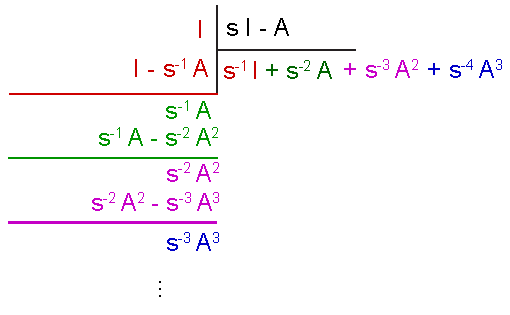
\includegraphics[width=\textwidth]{s_directdivision}
     \end{center}
 \end{minipage}
     \end{center}
%
If we follow the path we can find that 
%
\begin{align*}
\left( s I - A \right)^{-1} &= s^{-1} I + s^{-2} A + s^{-3} A^2 +
                              s^{-4} A^3 +  s^{-5} A^4 + 
  + \cdots
\\
\Psi(t) = \mathcal{L}^{-1} \left[ \left( s I - A \right)^{-1} \right] &= I + A t
  + A^2 \frac{t^2}{2} + A^3 \frac{t^3}{3 !} + A^4 \frac{t^3}{4 !} + 
                                                              \cdots =
                                                                        e^{A t}
\end{align*}
%
We can then find initial condition only response and impulse response
matrix of the system using $\Psi(t) = e^{A t}$
%
\begin{itemize}
\item Initial Condition Only Response : $x(t) = e^{A t} x_0$
\item Impulse Response Matrix :  $ G(t) = C e^{A t} B + D \delta(t) $
\end{itemize}
%
In that respect general solution can be written as
%
\begin{align*}
  x(t) &= e^{A t} x_0 + \int\limits_{0}^{t} e^{A ( t - \tau ) } B u(\tau) d
                  \tau
\\
  y(t) &= C e^{A t} x_0 + \int\limits_{0}^{t} C e^{A ( t - \tau ) } B u(\tau) d
                  \tau + D u(t)
\end{align*}


\subsection{DT State-Space to $z-$domain}

Note that a SS representation of an $n^{th}$ order DTI-LTI system has the from below.
%
\begin{align*}
  \mathrm{Let} \ x[k] &\in \mathbb{R}^n \ , \ y[k] \in \mathbb{R}^q \ ,\  u[k] \in
  \mathbb{R}^p , \\
  x[k+1] &= A x[k] + B u[k] , \\
  y[k] &= C x[k] + D u[k] , \\
  \mathrm{where} \ A &\in \mathbb{R}^{n \times n} \ , \ 
    B \in \mathbb{R}^{n \times p} \ ,\  C \in \mathbb{R}^{q \times n} \ , \ D \in \mathbb{R}^q
\end{align*}
%
In order to convert state-space to frequency domain, we start with taking the $Z-$transform of the 
both sides of the state-equation, where Z-transform of a unilateral (causal) discrete time signal $w[k]$ is given by 
%
\begin{align*}
  W(z) = \mathcal{Z} \lbrace w[k] \rbrace = \sum\limits_{k=0}^{\infty} w[k] z^{-k} 
\end{align*}
%
\begin{align*}
x[k+1] &= A x[k] + B u[k]
\\
z X(z) - z x[0] &= A X(z) + B U(z)
\\
z X(z) - A X(z) &= z x[0] +  B U(z)
\\
\left( z I - A \right) X(Z) &=  z x[0] +  B U(z)
\\
X(z) &= z \left( z I - A \right)^{-1} x[0] + \left( z I - A \right)^{-1} B U(z)
\end{align*}
%
I recommend to those of you not familiar with Z-transform operation on
difference equations to read \textit{shifting theorem} in EE402 Lecture Notes (Lecture
\# 2), indeed going over the whole Lecture would be very helpful. 

Now let's concentrate on the output equation
%
\begin{align*}
y[k] &= C x[k] + D u[k]
\\
Y(z) &= z C  \left( z I - A \right)^{-1} x[0] + \left[ C \left( z I - A \right)^{-1} B + D \right] U(z)
\end{align*}
%
where $z C  \left( s I - A \right)^{-1} x[0]$ corresponds to the initial-condition response and 
when $u[k]=0$ we have
%
\begin{align*}
Y(z) &=  \left[ C \left( z I - A \right)^{-1} B + D \right] U(z)
\\
G(z) &= C \left( z I - A \right)^{-1} B + D
\end{align*}
%
similar to the CT case $G(z)$ is called the \textbf{transfer function
  matrix}. Note that resultant frequency domain solution in DT systems
is very simlar to the solution in CT systems (except the initial
condition response). Without a big surprize state-space to transfer function related
definitions CT systems generally holds also for DT systems, Such as \textit{properness, poles,
  zeros} etc.



% **** This ENDS THE EXAMPLES. DON'T DELETE THE FOLLOWING LINE:
\end{document}
